%!TEX root = ../dokumentation.tex

\chapter{LIN-Bus}

Der \ac{LIN}-Bus wurde entwickelt, um eine kostengünstigere Alternative zum Low-Speed-CAN zu schaffen.
Es wurde von einem Konsortium mehrerer Automobilhersteller entwickelt und 2001 erstmals im Mercedes Benz SL eingesetzt.
\ac{LIN} dient der Vernetzung einzelner Teilbereiche eines Fahrzeugs als Subnetz zu \ac{CAN} und hat deswegen eine sehr geringe Datenrate und nur wenige Busteilnehmer (maximal 16).
Es besteht eine lineare Busstruktur und die einzelnen Knoten sind durch eine Eindrahtleitung verbunden. 
Eine vorgeschriebene Topologie existiert nicht, wobei es meist als lineare Busstruktur umgesetzt wird.
\begin{figure}[!htbp]
    \centering
    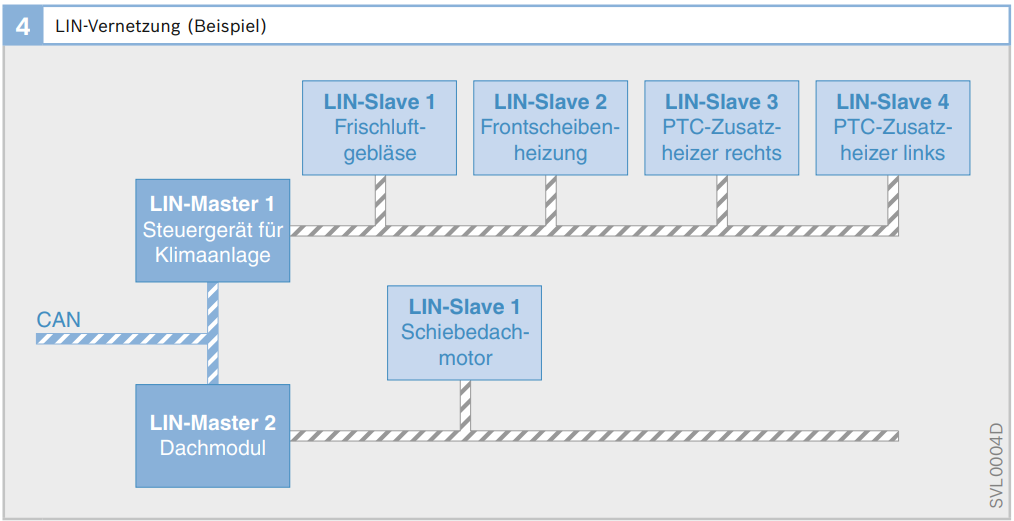
\includegraphics[width=0.5\linewidth]{own/LIN/Vernetzung_BAA111.png}
    \caption{Grafik Vernetzung bei LIN, Quelle: \cite{BAA2011, S.111}}
    \label{fig:Toleranzbaender}
\end{figure}


\section{Verwendungszweck}
\ac{LIN} wird hauptsächlich verwendet, um Sensoren und Aktoren in der Karosserieelektronik zu vernetzen, die nicht die Bandbreite von \ac{CAN} benötigen.
Dafür werden oft einzelne Elemente eines Autos mit einem eigenen Bus vernetzt.
Ein Beispiel dafür wäre ein Türmodul, welches mehrere Sensoren und Aktoren, wie die Verrieglung, Außenspiegelverstellung und Tasten für die Sitzverstellung, besitzt.

\section{Übertragungssystem}
    \subsection{Aufbau und Pegel}
    Als Übertragungsmedium wird bei \ac{LIN} eine unabgeschirmte Eindrahtleitung verwendet, die zwei Pegel annehmen kann.
    Der dominante Pegel (logisch 0) hat meist 0V, während der rezessive Pegel (logisch 1) üblicherweise der Batteriespannung entspricht.
    Der rezessive Pegel ist am Master mit  $1k\Omega$  und am Slave mit $30k\Omega$  abgesichert.
    Durch die Vielzahl an unterschiedlichen Anwendungszwecken und so auch Vernetzungen, akzeptiert \ac{LIN} einen sehr breiten Toleranzbereich beim Empfangen der Daten, damit auch mit Störsignalen noch gültige Signale empfangen werden können. 
    \begin{figure}[!htbp]
        \centering
        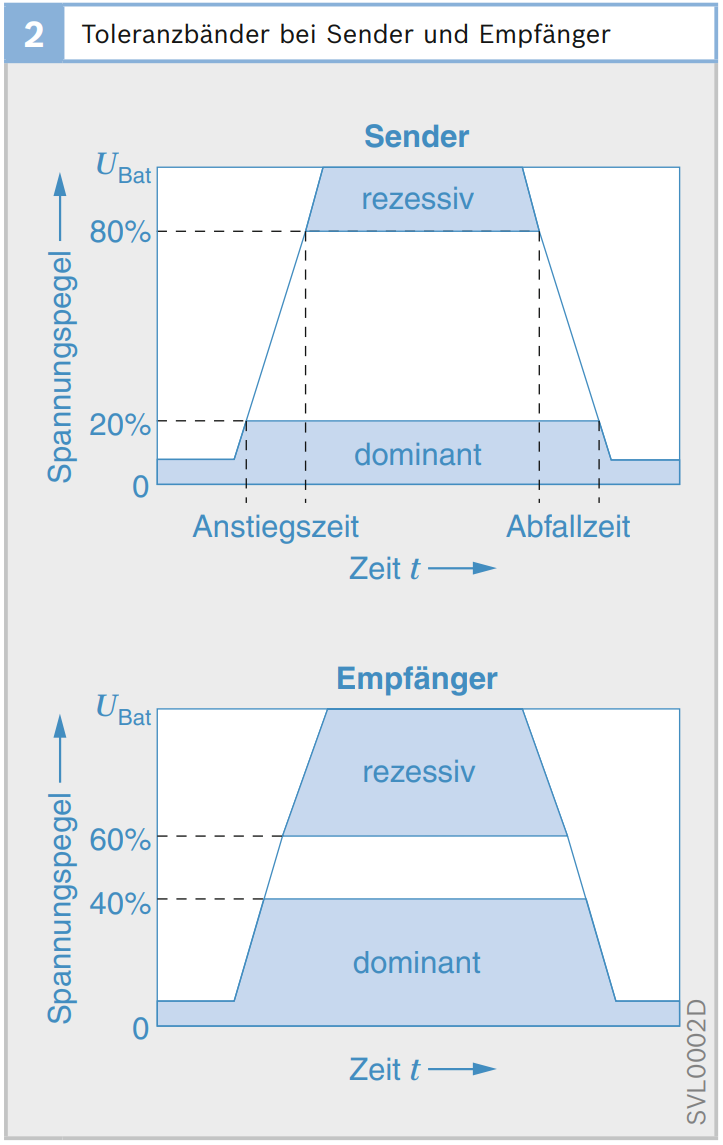
\includegraphics[width=0.3\linewidth]{own/LIN/ToleranzbänderSenderEmpfänger_BAA107.png}
        \caption{Grafik Toleranzbänder, Quelle: \cite{BAA2011, S.107}}
        \label{fig:Toleranzbaender}
    \end{figure}

    \subsection{Buszugriff}
    Der LIN-Bus verwendet das Master-Slave Verfahren, wobei Nachrichten entweder zwischen einem (Point-to-Point), mehreren (Multicast) oder allen (Broadcast) Slaves ausgetauscht werden.
    Es gibt für den Master mehrere Möglichkeiten eine Kommunikation zwischen Knoten zu initiieren.
    Die Erste ist, dass der Master der Slave nach Daten fragt (z.B. Messwerte oder Schalterzustände), eine Weitere wäre, dass der Master dem Slave eine Anweisung sendet (z.B. Verschließen der Tür).
    Außerdem kann der Master eine Kommunikation zwischen zwei Slaves initiieren. 

    \subsection{Datenrate}
    Die maximale Datenrate liegt bei 20kBit/s, da dies ein guter Kompromiss aus der Forderung nach einer hohen Flankensteilheit (Dauer, die der Spannungspegel zum Ansteigen braucht) zur Synchronisierung der Slaves und einer geringen Flankensteilheit zur Verbesserung des \acused{EMV}\ac{EMV}-Verhaltens ist.
    Als empfohlene Standardübertragungsrate wird meist 2,4kBit/s, 9,6kBit/s und 19,2kBit/s gewählt, sowie eine minimale Übertragungsrate von 1kBit/s um Timeouts zu vermeiden.
    Es ist eine Flankensteilheit mit $1 \text{ \it{bis} } 3 \frac{V}{\mu s}$ angegeben.


\section{LIN-Protokoll}
    \subsection{Frame}
    Beim \ac{LIN}-Protokoll werden die Daten in einen Frame eingebettet.
    Das zu sendende Paket startet mit dem Header (Botschaftskopf), in dem die Synchronisierung und die Nachrichtenidentifikation stattfindet.
    Dieses Paket wird von einer Response (Nachrichtenfeld) beantwortet. 
    \begin{figure}[!htbp]
        \centering
        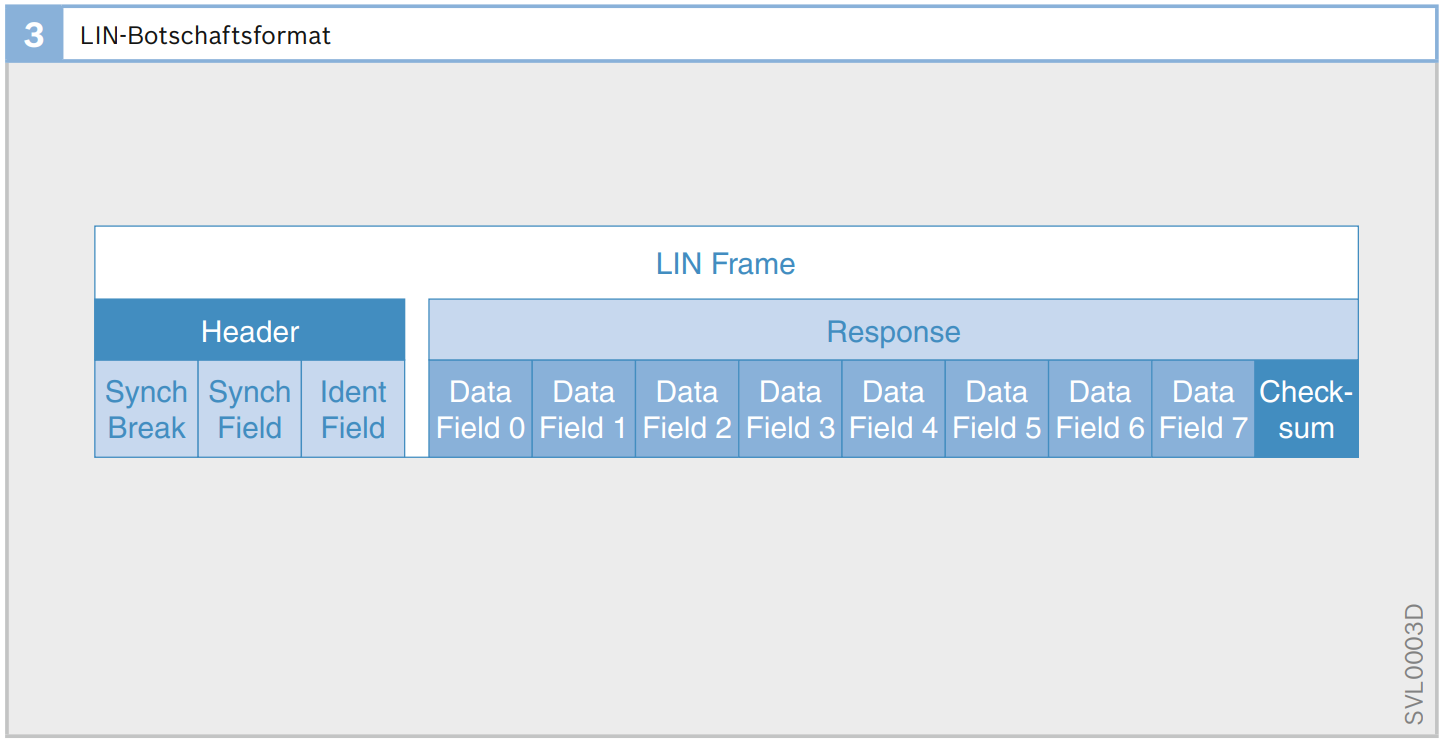
\includegraphics[width=0.5\linewidth]{own/LIN/Frame_BAA108.png}
        \caption{Grafik Frame, Quelle: \cite{BAA2011, S.108}}
        \label{fig:FrameLIN}
    \end{figure}

    \subsection{Synchronisierung}
    Zu Beginn einer Nachrichtenübertragung werden alle Clients synchronisiert. Dies wird benötigt, damit man eine große Spezifikation des Timings zu erreichen und somit kostengünstige Hardware ohne Quarzoszillatoren einsetzen kann.
    Der Master darf nicht mehr als $\pm 0,5\%$ vom Takt abweichen, während der Slave am Anfang der Synchronisation bis zu $15\%$ abweichen darf, wenn er am Ende der Synchronisation nicht mehr als $2\%$ vom Master abweicht.
    Für die Synchronisierung sendet der Master erst die Syncbreak (Synchronisierungspause), in dem 13 aufeinanderfolgende dominante Bits gesendet werden und ein rezessives Bit gesendet wird.
    Danach wird mit dem Syncfield (Synchronisierungsfeld) die Bitfolge 01010101 vom Master gesendet, damit die Slaves ihre Zeitbasis mit dem des Masters abgleichen und anpassen können.
    Somit sind alle Slaves mit dem Master synchronisiert.
    
    \subsection{Identifier}
    Das dritte Byte des Headers ist der Identifier der Nachricht.
    Diese ist parallel zum CAN-Bus auch eine inhaltsbasierte Adressierung und gibt Aufschluss über den Inhalt der Botschaft.
    Für die Akzeptanzfilterung prüfen alle am Bus angeschlossenen Knoten, ob sie die Botschaft empfangen, verarbeiten oder ignorieren wollen.
    Der Identifier besteht aus 6 Bit, wodurch 64 mögliche Identifier möglich sind.
    Allerdings sind 4 davon für systemrelevante Zwecke reserviert.
    Abgeschlossen wird der Identifier mit 2 Bit für die Prüfsumme des Identifier, damit es nicht zu einem Übertragungsfehler oder einer fehlerhaften Botschaftszuordnung kommt.
    
    \subsection{Response/Datenfeld}
    Im Datenfeld findet die eigentliche Übertragung der Daten statt.
    Der Slave erkennt aus dem Identifier, ob er angesprochen wird und sendet daraufhin die Antwort im Datenfeld zurück.
    Die Datenübertragung startet mit einem \ac{LSB}.
    Jedes einzelne Byte, dass übertragen werden soll, wird mit einem Startbit eingeleitet und mit einem Stoppbit abgeschlossen.
    Dies dient zur Neusynchronisation der Knoten, um Datenübertragungsfehler zu vermeiden.
    Auch bei \ac{LIN} wird die Datenübertragung durch das Errechnen, Senden und Vergleichen von Prüfsummen abgesichert. 
    
    \subsection{LDF-File}
    Das \ac{LIN} Description File dient dazu, Spezifikationen von Netzteilnehmern, Frames und Identifierer in einer Konfiguration festzuhalten.
    Es wird dadurch das komplette \ac{LIN}-Netzwerk konfiguriert, weshalb es auch Aufschluss über die gemeinsamen Schnittstellen zwischen den Komponenten in einem Automobil gibt.
    Zum Beispiel die Schnittstelle zwischen dem Auto und einem Automodul (z.B. eine Tür), dass von einem Zulieferer geliefert wird.
    Aus diesem \acused{LDF}\ac{LDF}-File können außerdem automatisch Daten in C generiert werden, die zur Implementierung von \ac{LIN} in den Steuergeräten verwendet werden.

    \subsection{Message Scheduling}
    Die Nachrichten werden bei \ac{LIN} gemäß der im \ac{LDF}-File vorhandenen Scheduling-Tabelle, festgelegten Reihenfolge und des Zeitrahmens übermittelt.
    Häufig benötigte Informationen können öfters in der Liste eingetragen werden und werden somit mehrfach abgearbeitet.
    Der Master arbeitet diese Liste von Anfang bis Ende ab und fängt danach wieder von vorne an.
    Damit ist das Übertragungsraster für jede Nachricht bekannt, dass gewährleistet, dass jede Übertragung vom Master initiiert wird. 
    Die Scheduling-Tabelle kann sich allerdings je nach Betriebszustand des Autos (z.B. Zündung an oder aus) verändern.
    Außerdem können beim weiterentwickelten \ac{LIN}2.0 Bus Daten auch nach Bedarf vom Master mit einem speziellen Identifier (Sporadic Frames) angefordert werden und Slaves können mit einem speziellen Identifier (Event Triggered Frames) Ereignisse melden.

    \subsection{Sleep Mode}
    Auch beim LIN-Bus existiert einen Sleep-Modus, um den Stromverbrauch zu senken.
    Dieser kann entweder durch einen speziellen Identifier (60) als Kommando vom Master initiiert werden oder die Slaves gehen selbstständig in den Sleep Mode nach einer Übertragungslücke von 4 Sekunden.
    Zum Aufwecken wird vom Master ein Wake-Up-Signal in Form von 128 Datenbytes geschickt und alle Slaves müssen nach 4-64 Bitzeiten initialisiert sein und auf den Master reagieren können.